\begin{longtable}{|m{3cm}|m{9cm}|m{2.5cm}|}
\hline
Identificateur & Descritption & image \\
\hline
Avion  & Schema représentant un avion & \includegraphics[width=2.5cm]{img/Avion.pdf} \\
\hline
bagages  & Schema représentant une valise & 
\includegraphics[width=2.5cm]{img/bagages.pdf} \\
\hline
Terminal  & La lettre T suivie du numéro du Terminal & 
\includegraphics[width=2.5cm]{img/Terminal.pdf} \\
\hline
Hall  & La lettre H suivie du numéro du Hall & 
\includegraphics[width=2.5cm]{img/Hall.pdf} \\
\hline
caroussel  & Schema représentant un caroussel & 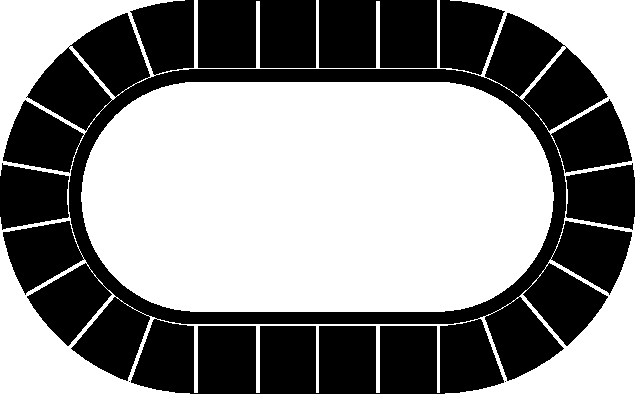
\includegraphics[width=2.5cm]{img/caroussel.pdf} \\
\hline
chariot  & Schema représentant un chariot & 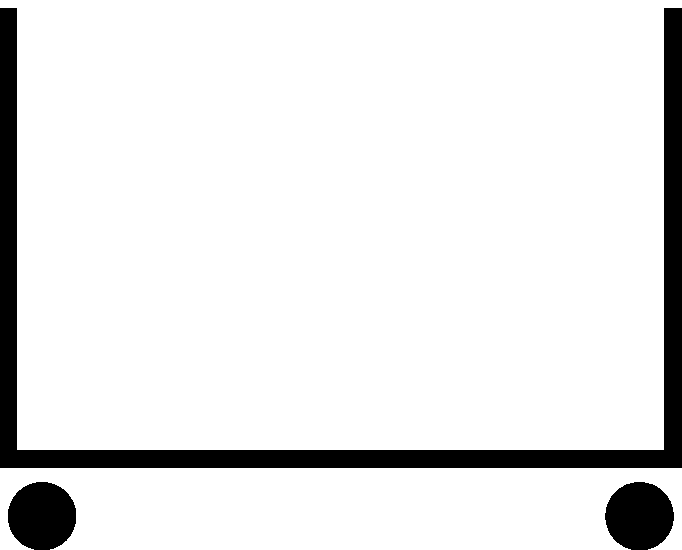
\includegraphics[width=2.5cm]{img/chariot.pdf} \\
\hline
rechargement-batterie  & Schema représentant un chariot munie d'une prise electrique & 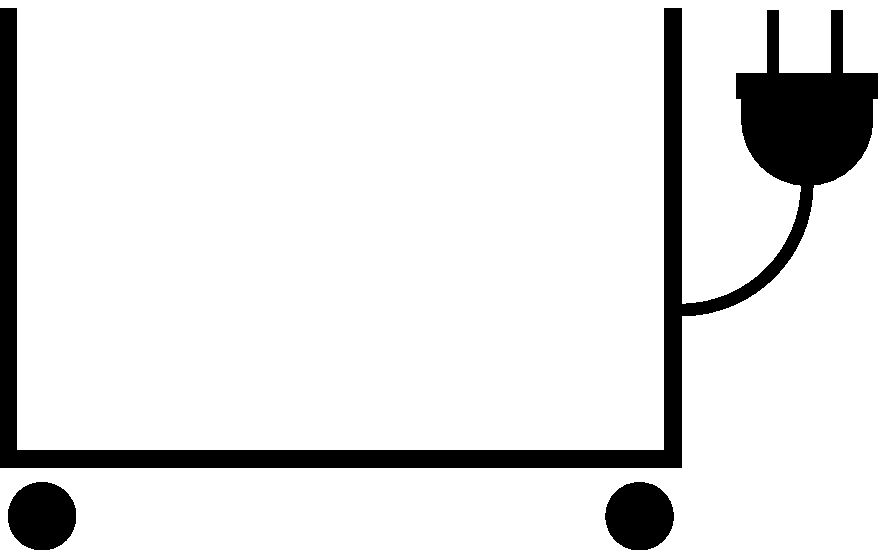
\includegraphics[width=2.5cm]{img/rechargement-batterie.pdf} \\
\hline
Reparation-chariot  & Un schema représentant un chariot surmonté de deux outils symbolisant la réparation  & 
\includegraphics[width=2.5cm]{img/Reparation-chariot.pdf} \\
\hline
Chariot-elevateur  & Schema représentant un chariot élévateur & 
\includegraphics[width=2.5cm]{img/Chariot-elevateur.pdf} \\
\hline
tapis-roulant  & Schema représentant un tapis roulant & 
\includegraphics[width=2.5cm]{img/tapis-roulant.pdf} \\
\hline
tapis-roulant-dessus  & Schema représentant un tapis roulant vue de dessus & 
\includegraphics[width=2.5cm]{img/tapis-roulant-dessus.pdf} \\
\hline
train  & Schema reprénsentant un train & 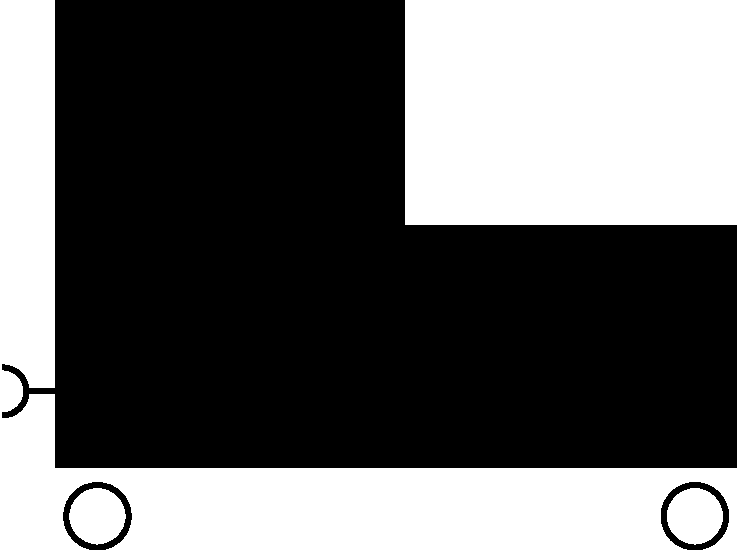
\includegraphics[width=2.5cm]{img/train.pdf} \\
\hline
wagonnet  & Schema représentant un wagonnet & 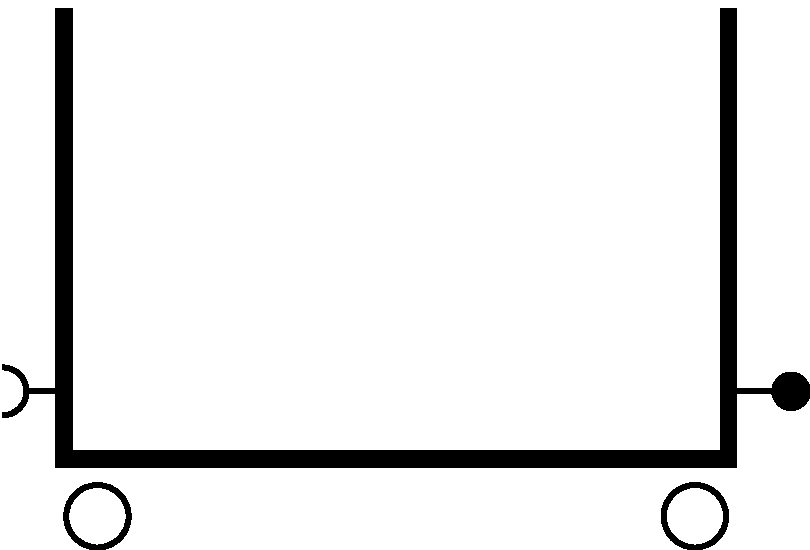
\includegraphics[width=2.5cm]{img/wagonnet.pdf} \\
\hline
train\_wagonnet & Schema représentant un train suivi de wagonnets & 
\includegraphics[width=2.5cm]{img/train_wagonnets.png} \\
\hline
logo  & Logo du logiciel SGBag & 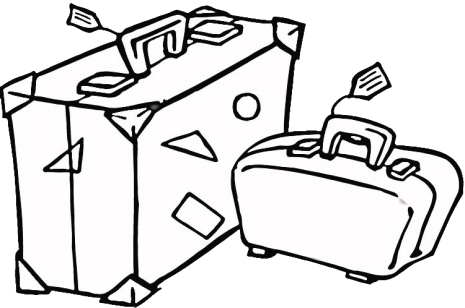
\includegraphics[width=2.5cm]{img/logo.png} \\
\hline
ok  & Symbole universel de validation & 
\includegraphics[width=2.5cm]{img/ok.png} \\
\hline
cancel  & Croix de saint andré & 
\includegraphics[width=2.5cm]{img/cancel.png} \\
\hline
undo  & Schema indiquant l'annulation de la dernière action & 
\includegraphics[width=2.5cm]{img/undo.png} \\
\hline
redo  & Schema indiquand le retour de la dernière action annulé & 
\includegraphics[width=2.5cm]{img/redo.png} \\
\hline
play  & Schema universel de lecture & 
\includegraphics[width=2.5cm]{img/play.png} \\
\hline
pause  & Schema universel de pause & 
\includegraphics[width=2.5cm]{img/pause.png} \\
\hline
stop  & Schema universel de stop & 
\includegraphics[width=2.5cm]{img/stop.png} \\
\hline
save  & Schema de disquette indiquant la sauvegarde & 
\includegraphics[width=2.5cm]{img/save.png} \\
\hline
saveas  & Schema de disquette surmonté d'un crayon indiquant une nouvelle souvegarde & 
\includegraphics[width=2.5cm]{img/saveas.png} \\
\hline
open  & Schema de dossier ouvert & 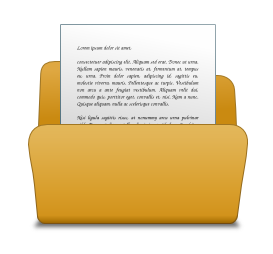
\includegraphics[width=2.5cm]{img/open.png} \\
\hline
loupe  & Schema d'une loupe avec un signe plus ou un signe moins au niveau du verre & 
\includegraphics[width=2.5cm]{img/loupe.png} \\
\hline
ajouter  & Croix grecque & 
\includegraphics[width=2.5cm]{img/ajouter.png} \\
\hline
alert  & Panneau de signalisation indiquant un danger & 
\includegraphics[width=2.5cm]{img/alert.png} \\
\hline
logout  & Symbole universel de changement d'état d'alimentation & 
\includegraphics[width=2.5cm]{img/logout.png} \\
\hline

\end{longtable}

